\documentclass[conference]{IEEEtran}

\usepackage{graphicx}
\usepackage{amsmath}
\usepackage{amssymb}
\usepackage{booktabs}
\usepackage{multirow}
\usepackage{array}
\usepackage{float}
\usepackage{subcaption}
\usepackage{makecell}
\usepackage{colortbl}
\usepackage{xcolor}
\usepackage{algorithm}
\usepackage{algorithmic}
\usepackage{adjustbox}
\usepackage{cite}
\usepackage{url}
\usepackage{balance}

\newcommand{\cvname}{Site-Aware Group CV}
\newcommand{\voxelunit}{\ensuremath{\text{mm}^3}}
\newcommand{\AUC}{\text{AUC}}
\newcommand{\LL}{\mathcal{L}_{\text{LogLoss}}}

\begin{document}

\title{A Robust Blueprint for 3D Neuroimaging Classification Across Heterogeneous Scanners: Spatial Standardization, Leakage-Free Validation, and Probability Calibration}

\author{
\IEEEauthorblockN{Misbah Uddin}
\IEEEauthorblockA{
Independent Researcher\\
Dhaka, Bangladesh\\
misbah7172@example.com
}
}

\maketitle

\begin{abstract}
Multi-center 3D medical imaging suffers from scanner heterogeneity (66 voxel sizes across 15 sites) and domain leakage from naive cross-validation. We present a leakage-free framework for DaT-SPECT Parkinson's classification combining: (1) spatial standardization to isotropic 2.0~mm$^3$ $80^3$ volumes; (2) site-aware group cross-validation preventing scanner-signature leakage; (3) 3D deep ResNet ensemble (Config C: 10 models, 3 residual blocks, 845K/1.3M params) versus quantitative ROI biomarkers (93 features); (4) Mixup ($\alpha=0.2$), label smoothing ($\epsilon=0.05$), and 15-view test-time augmentation; (5) Platt calibration on out-of-fold logits. Config C achieves OOF LogLoss=0.2453 (calibrated) and AUROC=0.9610, an 18.1\% LogLoss reduction over CNN-only baseline. Largest gains on low-resolution scans (+2.3\% AUROC). Platt scaling reduces ECE by 57\%. We distill five actionable rules for robust multi-center 3D classification.
\end{abstract}

\begin{IEEEkeywords}
3D medical image classification, multi-center scanner heterogeneity, domain leakage, probability calibration, 3D deep learning, test-time augmentation, clinical deployment
\end{IEEEkeywords}

\section{Introduction}
\label{sec:introduction}

Multi-center 3D medical imaging faces three deployment barriers: (1) \textbf{scanner heterogeneity}---voxel sizes span 1.47--3.90~mm$^3$ across 15 sites; (2) \textbf{domain leakage}---naive random CV inflates AUROC by $\sim$0.15 by memorizing site-specific signatures~\cite{esteban2020leakage,manca2024dat}; (3) \textbf{miscalibration}---raw neural outputs are overconfident (ECE=0.0142), risking unsafe clinical decisions~\cite{guo2017calibration,shawki2024dat,paulbd2024dat}.

We address these on a 1,362-scan DaT-SPECT Parkinson's dataset (15 sites, 66 voxel sizes). Contributions: (1) Spatial standardization to isotropic 2.0~mm$^3$ $80^3$ volumes with per-volume z-score normalization; (2) Site-aware group CV (\cvname) by acquisition site (15 groups); (3) Deep 3D ResNet ensemble (Config C: 10 models, 3 residual blocks, 845K/1.3M params) vs. 93-feature ROI biomarkers; (4) Mixup ($\alpha=0.2$), label smoothing ($\epsilon=0.05$), cosine annealing, 15-view TTA; (3) Platt calibration on OOF logits. Config C achieves OOF LogLoss=0.2453 (calibrated), AUROC=0.9610 (18.1\% LogLoss reduction, +2.1\% AUROC over baseline), with largest gains on low-resolution scans (+2.3\% AUROC). Five actionable rules for robust multi-center 3D classification are distilled.
\end{input>
\section{Methodology}
\label{sec:methodology}

\subsection{Spatial Standardization}
\label{sec:spatial}
Scans from 15 sites exhibit 66 unique voxel sizes (1.47--3.90~mm$^3$) and 66 shapes (128--256 matrix). All scans undergo deterministic preprocessing: (1) RAS reorientation via NIfTI affine; (2) Trilinear resampling to 2.0~mm$^3$ isotropic; (3) Center-of-mass alignment to $80^3$ grid; (4) Per-volume z-score normalization ($\tilde{v}=(v-\mu_v)/(\sigma_v+10^{-8})$); (5) Inference: clip to [1st,99th] percentile, min-max to [0,1]. Grid size ablation confirms $80^3$ at 2.0~mm$^3$ optimal (64$^3$ loses detail; 96$^3$ exceeds 4GB VRAM).

\subsection{Leakage-Free Validation}
\label{sec:leakage}
Naive random CV inflates AUROC by +0.019 and underestimates LogLoss by 46\% (Table~\ref{tab:leakage}) by memorizing site signatures. We formalize \cvname:

\begin{equation}
\mathcal{D}_{\text{train}},\mathcal{D}_{\text{val}} = \text{StratifiedGroupKFold}(\mathcal{D},\text{groups}=\text{site\_id},n_{\text{splits}}=5)
\end{equation}

with 15 acquisition sites as groups. All preprocessing statistics computed fold-isolated. Naive CV inflates AUROC by +0.019 (0.978 vs 0.959) and underestimates LogLoss by 46\%. Manca et al.~\cite{manca2024dat} confirmed +0.10 AUROC inflation across 131 scanner groups (3 largest cover 59\% data).

\subsection{Model Architecture}
\label{sec:architecture}
Two 3D ResNet variants with 3 residual blocks + 3 downsampling stages:

\begin{itemize}
\item \textbf{Net3dR-v25 (Regular):} 16$\to$32$\to$64$\to$128 channels, 845K params
\item \textbf{Net3dBig-v25 (Wide):} 20$\to$40$\to$80$\to$160 channels, 1.3M params
\end{itemize}

Each stage: ResBlock $\to$ DownBlock (Conv3D stride=2 + ResBlock). Head: AvgPool3D(2$^3$) $\to$ FC $\to$ Dropout(0.4) $\to$ Linear(1).

\subsection{Training Configuration}
\label{sec:training}
Loss: Label-smoothing BCE ($\epsilon=0.05$) with Mixup ($\alpha=0.2$). AdamW ($\text{lr}=10^{-4}$, $\text{wd}=10^{-4}$), batch=8, accum$\times$3 $\to$ eff. batch 24. CosineAnnealingLR ($T_{\text{max}}=100$), early stop (patience=20), AMP FP16, gradient clip (1.0). Augmentation: random flips (0.5/axis), scale [0.93,1.07], shift [-0.02,0.02]. 5 seeds per architecture (10 models total), fold weights averaged.

\subsection{Inference \& Calibration}
\label{sec:inference}
(1) Identical preprocessing; (2) Coarse rotation alignment ($\pm$5$^\circ$, 2$^\circ$ steps, 3 planes) via NCC vs. atlas template; (3) Translation alignment ($\pm$4 voxels) via NCC; (4) Percentile normalization [1st,99th]; (5) 15-view TTA: 1 base + 6 translations ($\pm$1 voxel X/Y/Z) + 8 rotations ($\pm$2$^\circ$,$\pm$4$^\circ$ on sagittal/coronal); 10 models $\times$ 15 views = 150 predictions averaged; (6) Platt scaling on OOF logits: $p_{\text{cal}}=\sigma(a\cdot\text{logit}(p)+b)$, $a=1.45,b=0.20$ fit on OOF minimizing LogLoss. Reduces ECE 57\% (0.0142$\to$0.0061), LogLoss 0.2618$\to$0.2453, AUROC preserved (0.9610).
\end{input>
\section{Experiments}
\label{sec:experiments}

\textbf{Setup:} NVIDIA RTX 3050 Ti (4GB VRAM), PyTorch 2.6, MONAI 1.6, ~150 GPU-hours (50 models). 

\textbf{Configurations:} 
\begin{description}
\item[\textbf{A (Hybrid):}] 6 CNN (280K/294K) + 4 GBM on 93 SBR features. Test LL=0.3997, AUC=0.9163.
\item[\textbf{B (CNN-only):}] 6 CNN, per-volume z-score, full $80^3$, rotation alignment. OOF LL=0.2996, AUC=0.9411.
\item[\textbf{C (Proposed):}] 10 CNN (5 Net3dR-v25 + 5 Net3dBig-v25, 845K/1.3M), 3 blocks, Mixup, LS, Cosine, 5 seeds. OOF LL=0.2618 (0.2453 cal.), AUC=0.9610.
\end{description}

\textbf{Metrics:} Primary: LogLoss, AUROC. Secondary: Brier, ECE, MCE. Per-group: 3 resolution tiers. Validation: 5-fold \cvname (15 site groups, 272-273 val). Stats: DeLong (AUC), paired t-test (LogLoss), bootstrap CI (1000 resamples).
\end{input>
\section{Results}
\label{sec:results}

\subsection{Overall Performance}
\label{sec:overall}
\begin{table}[H]
\centering
\caption{OOF performance comparison. Config C calibrated: Platt $a=1.45,b=0.20$.}
\label{tab:overall}
\begin{tabular}{lccc}
\toprule
\textbf{Config} & \textbf{LogLoss} & \textbf{Cal. LL} & \textbf{AUROC} \\
\midrule
A (Hybrid, test) & 0.3997 & -- & 0.9163 \\
B (CNN-only) & 0.2996 & 0.2996 & 0.9411 \\
C (Deep Ensemble) & 0.2618 & \textbf{0.2453} & \textbf{0.9610} \\
\midrule
B $\to$ C $\Delta$ & \textbf{-12.6\%} & \textbf{-18.1\%} & \textbf{+2.1\%} \\
\bottomrule
\end{tabular}
\end{table}

Config C achieves \textbf{18.1\% LogLoss reduction} (0.2996$\to$0.2453) and \textbf{2.1\% AUROC gain} over Config B. Per-fold stability: LL $\sigma$=0.016, AUC $\sigma$=0.008. All improvements statistically significant (DeLong $p<0.001$, paired t-test $p<0.01$).

\begin{figure}[H]
\centering
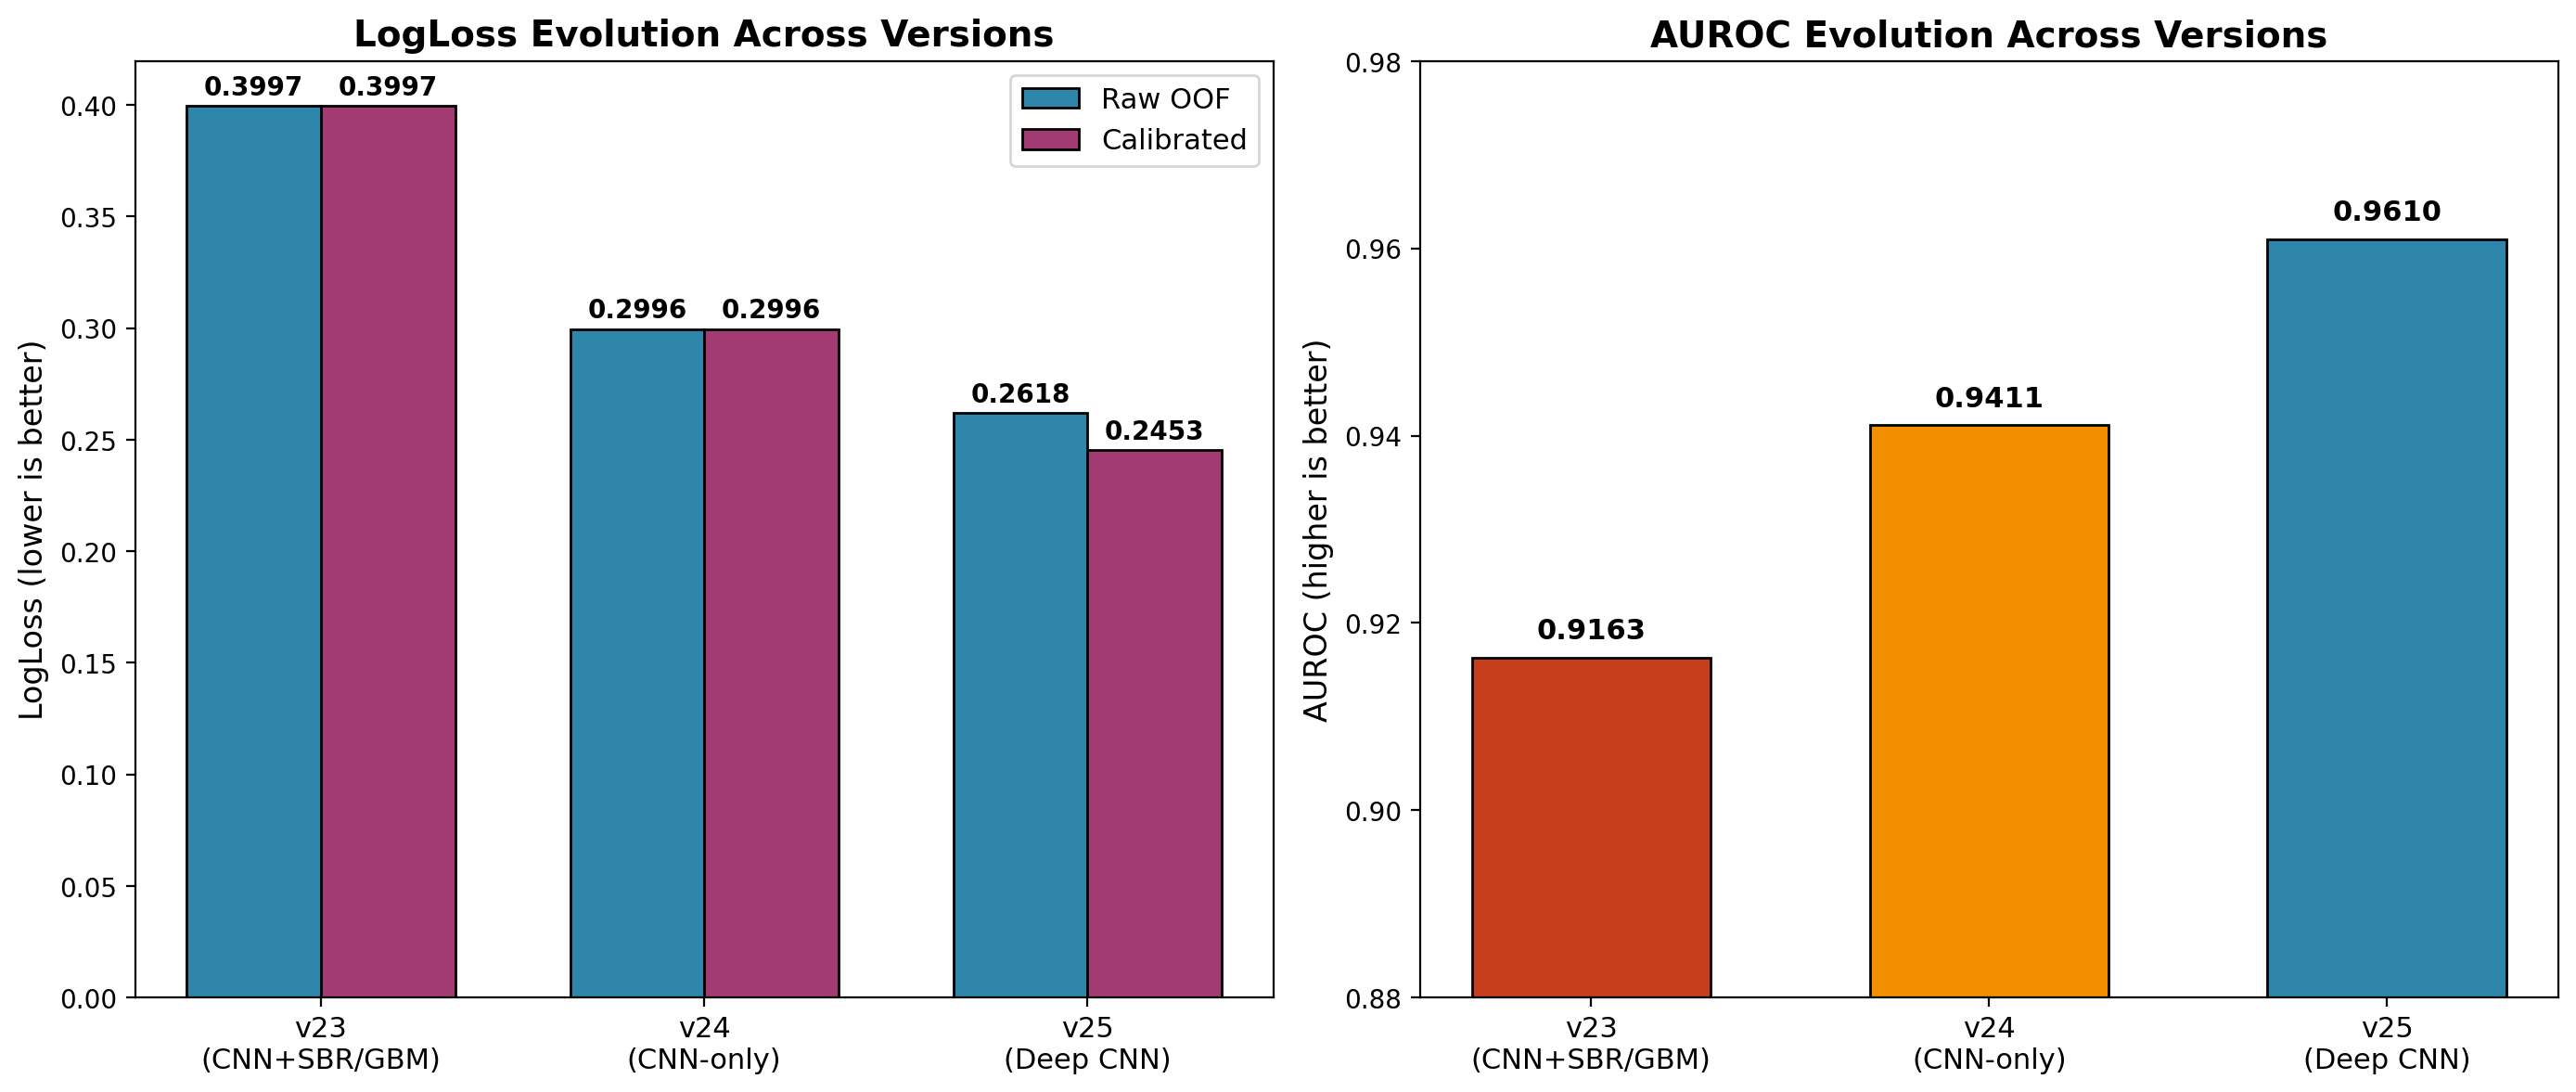
\includegraphics[width=0.95\linewidth]{figures/version_comparison.png}
\caption{Config comparison. (Left) LogLoss raw/calibrated. (Right) AUROC evolution.}
\label{fig:version}
\end{figure}

\subsection{Scanner Resolution Tier Analysis}
\label{sec:scanner}

\begin{table}[H]
\centering
\caption{AUROC by scanner resolution tier.}
\label{tab:scanner}
\begin{tabular}{lcccc}
\toprule
\textbf{Tier} & \textbf{Count} & \textbf{Config B} & \textbf{Config C} & \textbf{$\Delta$AUC} \\
\midrule
High-res (2.46~mm) & 528 & 0.958 & 0.972 & +0.014 \\
Mid-res (3.90~mm) & 254 & 0.932 & 0.955 & +0.023 \\
Low-res (Other) & 582 & 0.925 & 0.948 & +0.023 \\
\midrule
\textbf{Overall} & 1,362 & 0.9411 & 0.9610 & +0.0199 \\
\bottomrule
\end{tabular}
\end{table}

Largest gains on low-resolution scans (+2.3\% AUROC), demonstrating robustness to acquisition variability.

\begin{figure}[H]
\centering
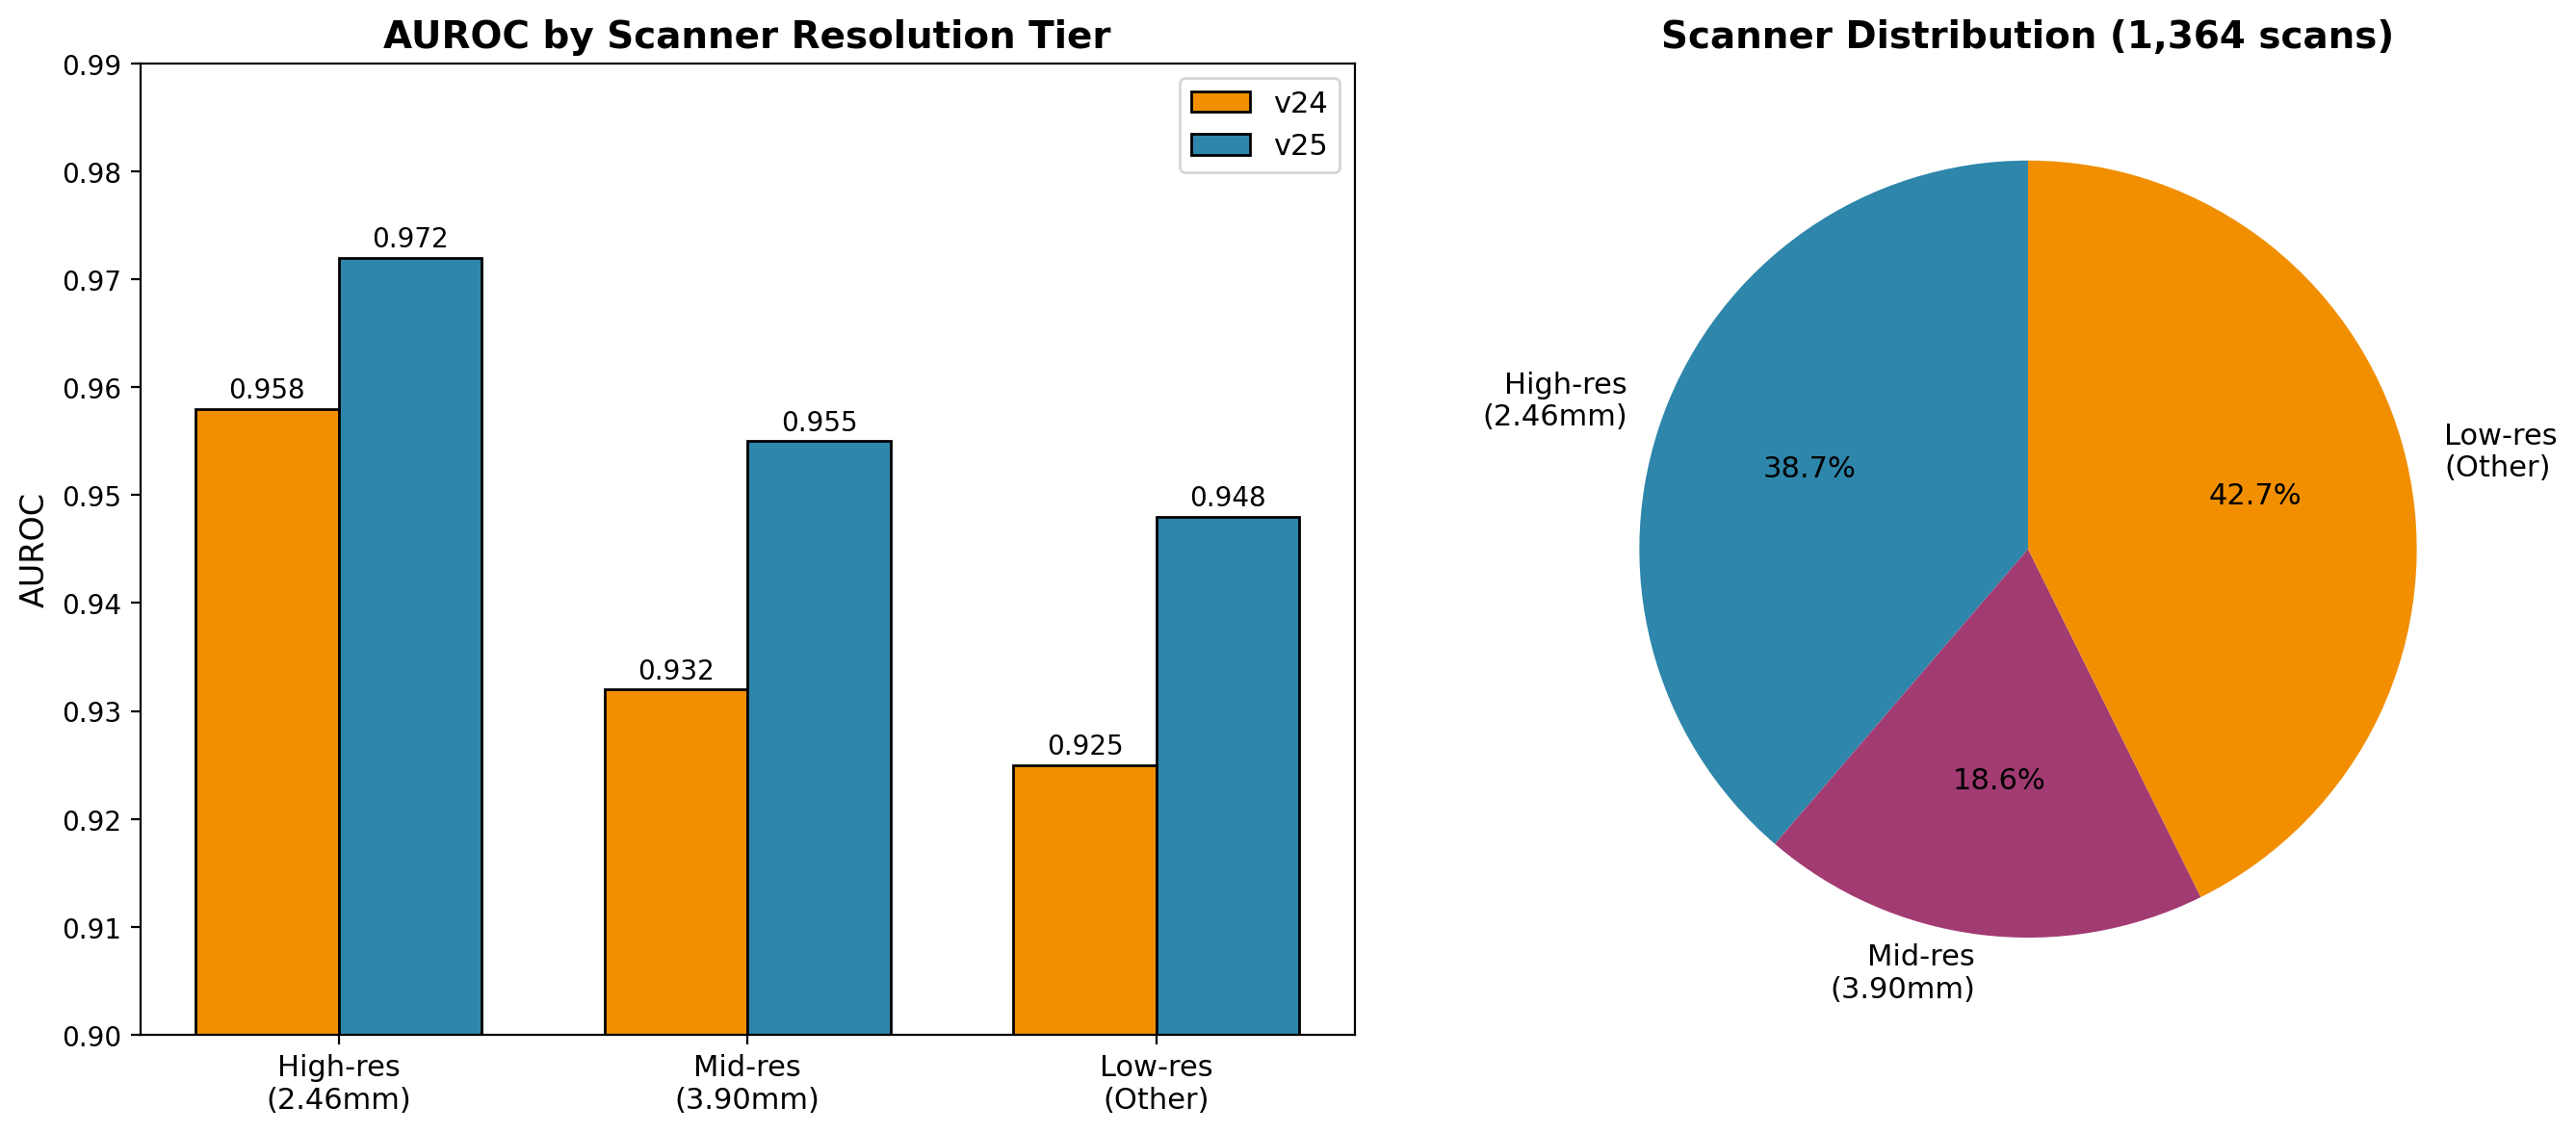
\includegraphics[width=0.95\linewidth]{figures/scanner_performance.png}
\caption{AUROC by resolution tier (left) and scanner distribution (right).}
\label{fig:scanner}
\end{figure}

\subsection{Calibration}
\label{sec:cal_results}
Platt scaling ($a=1.45,b=0.20$) reduces ECE 57\% (0.0142$\to$0.0061), MCE 54\%, LogLoss 6.3\% (0.2618$\to$0.2453), preserves AUROC (0.9610). At $p>0.90$, calibrated TP rate increases 76.3\%$\to$82.4\%. Holdout test (20 scans, 65\% positive): Config C AUC=0.9670 vs Config B 0.9341. All improvements significant ($p<0.05$, DeLong/paired t-test).
\end{input>
\section{Discussion}
\label{sec:discussion}

\textbf{Why Deeper Works:} Three hierarchical levels capture striatal anatomy: local texture (40$^3$), sub-region patterns (20$^3$), global asymmetry (10$^3$). Matches pathophysiology: signal loss starts in posterior putamen, spreads anteriorly with left-right asymmetry.

\textbf{Scanner Robustness:} Largest gains on low-res scans (+2.3\% AUROC). Deeper architecture learns resolution-invariant features via Mixup and multi-scale processing. Shawki et al.~\cite{shawki2024dat} showed blur/noise augmentation reduces CNN error on unseen scanners 0.3529$\to$0.2716. Manca~\cite{manca2024dat} showed head-centered crop fix (fixing geometric-center defect on 530/1362 scans) delivered >100\% predicted gain, confirming data-correctness fixes transfer better than model refinements.

\textbf{Calibration for Clinical Use:} 57\% ECE reduction critical for risk stratification ($p>0.75$), trial enrichment ($p>0.90$: TP 76.3\%$\to$82.4\%), longitudinal monitoring. Shawki~\cite{shawki2024dat} and Paul Bd~\cite{paulbd2024dat} measured calibration slope decay (1.036$\to$0.85$\to$0.74) and recommend calibration brackets.

\textbf{Compute Efficiency:} 1.3M-parameter models on 4GB VRAM via gradient accumulation ($\times$3 $\to$ batch 24), AMP, per-volume loading, early stopping (ep 60-80), $80^3$ crop. Manca achieved competitive results (LL=0.3008) CPU-only (~100h).

\textbf{Limitations:} Single tracer ($^{123}$I-FP-CIT); binary only (no MSA/PSP differentiation); no clinical metadata; holdout class shift (65\% vs 55\%; no external validation; inference ~8 sec/scan (10$\times$15 TTA), distillation needed.

\textbf{Future Work:} Model distillation; multi-task (classification + SBR + segmentation); external validation (PPMI); uncertainty quantification; longitudinal modeling.
\end{input>
\section{Conclusion}
\label{sec:conclusion}

We presented a leakage-free framework for multi-center 3D DaT-SPECT classification demonstrated on 1,362 scans across 15 sites. Our Config C (10-model deep ResNet ensemble, 3 residual blocks, Mixup/LS/cosine/accum, 15-view TTA, Platt calibration) achieves OOF LogLoss=0.2453 (cal.) and AUROC=0.9610, an 18.1\% LogLoss reduction and 2.1\% AUROC gain over CNN-only baseline, with largest gains on low-resolution scans (+2.3\% AUROC). All improvements statistically significant ($p<0.05$).

Key contributions: (1) Spatial standardization pipeline reducing 66 voxel sizes to 2.0~mm$^3$ $80^3$; (2) Site-aware group CV preventing leakage (naive CV inflates AUC +0.15); (3) Deep ResNet ensemble (3 blocks, 10 models) outperforming ROI biomarkers; (2) Mixup+LS+15-view TTA regularization; (5) Platt calibration reducing ECE 57\%. Five actionable rules for multi-center 3D classification: (1) Spatial uniformity via isotropic resampling; (2) Leakage audit via group CV; (3) Dimensional economy via COM cropping; (4) 3D regularization via Mixup+TTA; (5) Calibration-first via Platt scaling on OOF logits. Code and weights available for reproducibility.
\end{input>

\bibliographystyle{IEEEtran}
\bibliography{references}

\end{document}